\documentclass[12pt]{article}
\usepackage[letterpaper, margin=1in]{geometry}
\usepackage{graphicx}
\graphicspath{{./images/}}
\usepackage{amsmath}
\title{ELECENG 2CJ4 Lab 4}
\author{Raeed Hassan \\ hassam41 \\  \\ L01 \\ McMaster University}
\usepackage{enumitem}
\begin{document}
\maketitle
\pagebreak
\begin{enumerate}[label=\alph*)]
    \item The measured values for $V_{sat+}$ and $V_{sat-}$ are $V_{sat+} = 7.1378$ and $V_{sat-} = -7.13792$. The calculated values for $V_{th+}$ and $V_{th-}$ are $V_{th+} = \frac{R_2}{R_1+R_2}V_{sat+} = 7.1378\left(\frac{10k}{35k}\right) = 2.039V$ and $V_{th-} = \frac{R_2}{R_1+R_2}V_{sat-} = -7.13792\left(\frac{10k}{35k}\right) = -2.039V$.
    \item The waveforms for $v_c(t)$ and $v_{out}(t)$ for $C = 10nF, R_3 = 100k\Omega$ can be seen in Figure \ref{Fig:4bC10R100}. The period was measured to be approximately 500$\mu$s (2 kHz). The theoretical period was calculated to be $T = RC \left( \ln\frac{V_{sat+}-V_{th-}}{V_{sat+}-V_{th+}} + \ln\frac{V_{sat-}-V_{th+}}{V_{sat-}-V_{th-}} \right) = 0.001175 \approx 1175\mu\text{s}$ (851 Hz). The calculated theoretical value was over double the measured period.  
    \begin{figure}[h!]
        \centering
        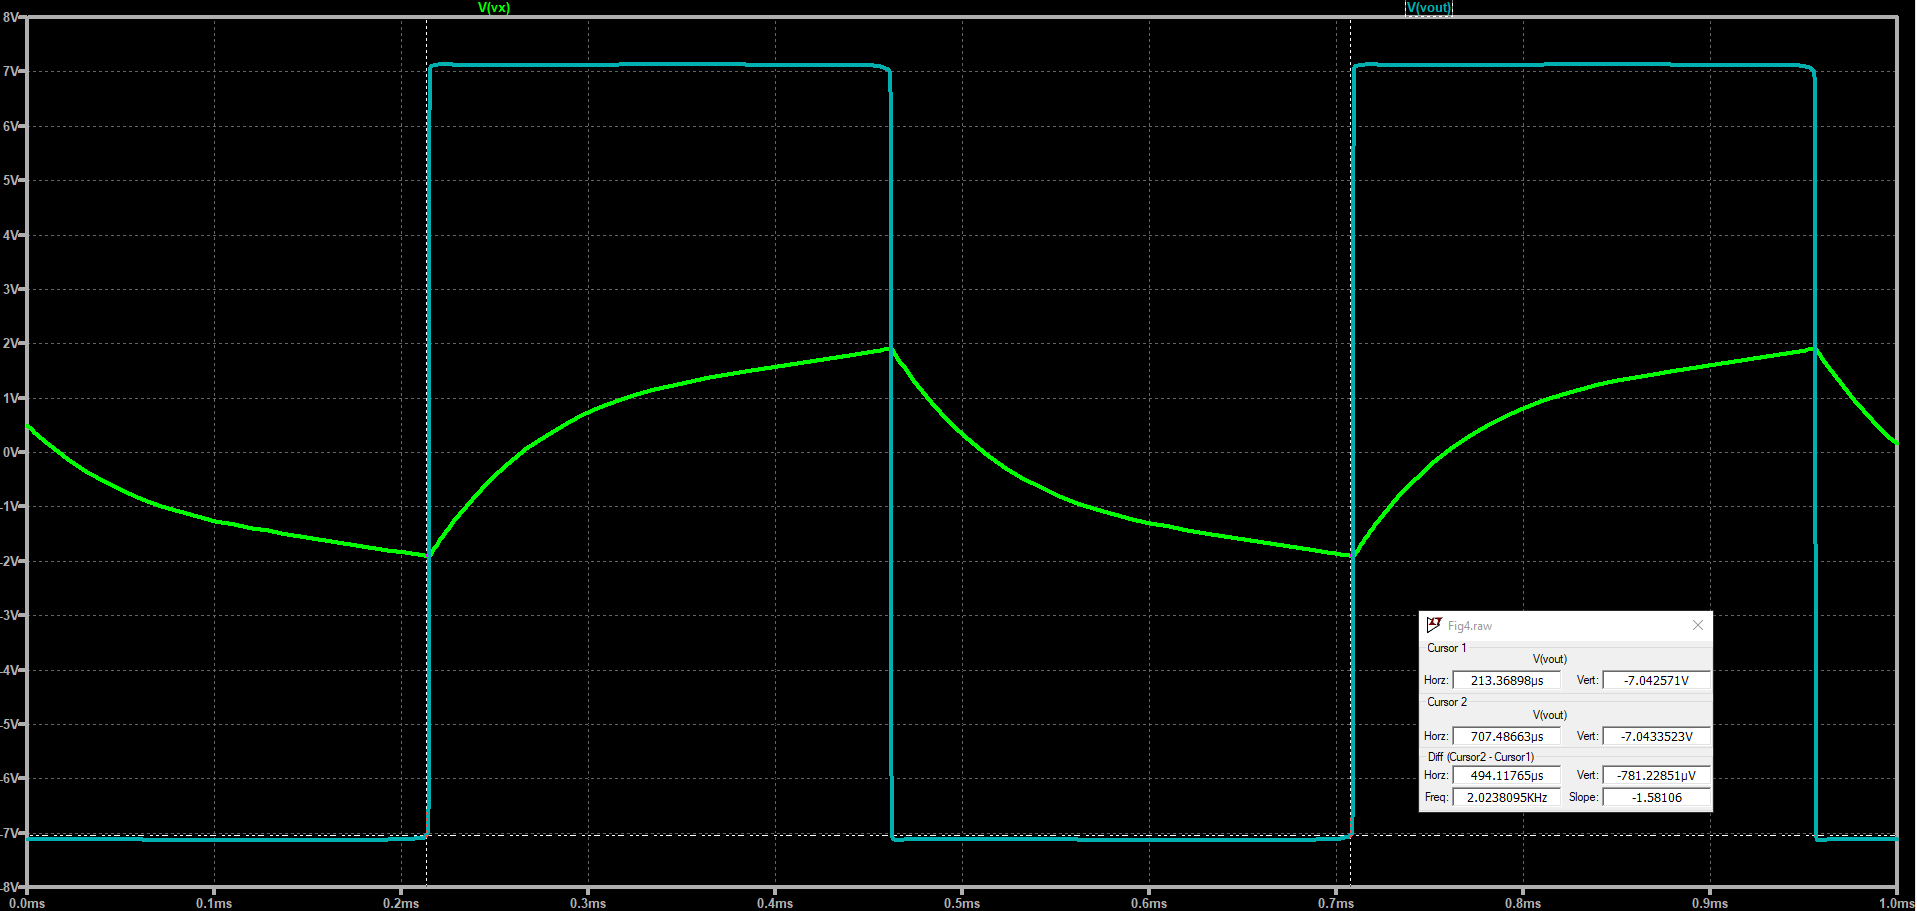
\includegraphics[width=0.86\textwidth]{4bC10R100.png}
        \caption{$v_c(t)$ (green) and $v_{out}(t)$ (cyan) for $C = 10nF, R_3 = 100k\Omega$}
        \label{Fig:4bC10R100}
    \end{figure}
    \item The waveforms for $v_c(t)$ and $v_{out}(t)$ for $C = 10nF, R_3 = 10k\Omega$ can be seen in Figure \ref{Fig:4bC10R10}. The period was measured to be approximately 94$\mu$s (10.7 kHz).
    \begin{figure}[h!]
        \centering
        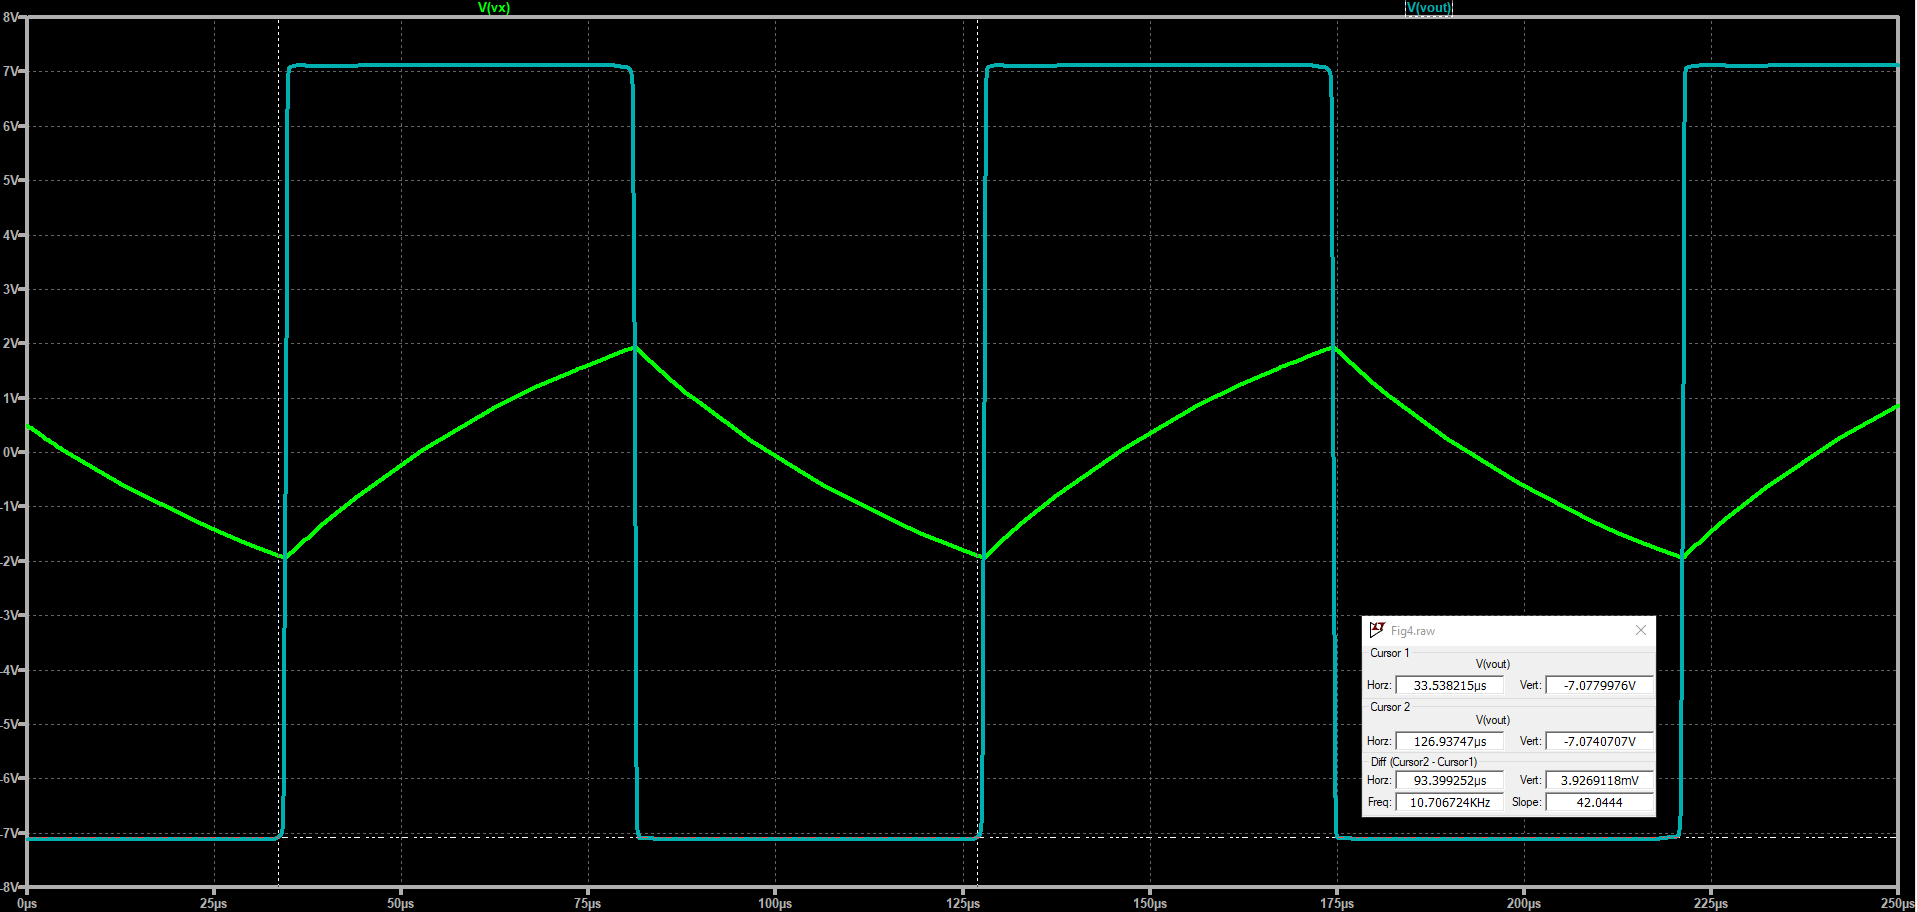
\includegraphics[width=0.86\textwidth]{4bC10R10.png}
        \caption{$v_c(t)$ (green) and $v_{out}(t)$ (cyan) for $C = 10nF, R_3 = 10k\Omega$}
        \label{Fig:4bC10R10}
    \end{figure} \\
    The waveforms for $v_c(t)$ and $v_{out}(t)$ for $C = 100nF, R_3 = 100k\Omega$ can be seen in Figure \ref{Fig:4bC100R100}. The period was measured to be approximately 5ms (200 Hz).
    \begin{figure}[h!]
        \centering
        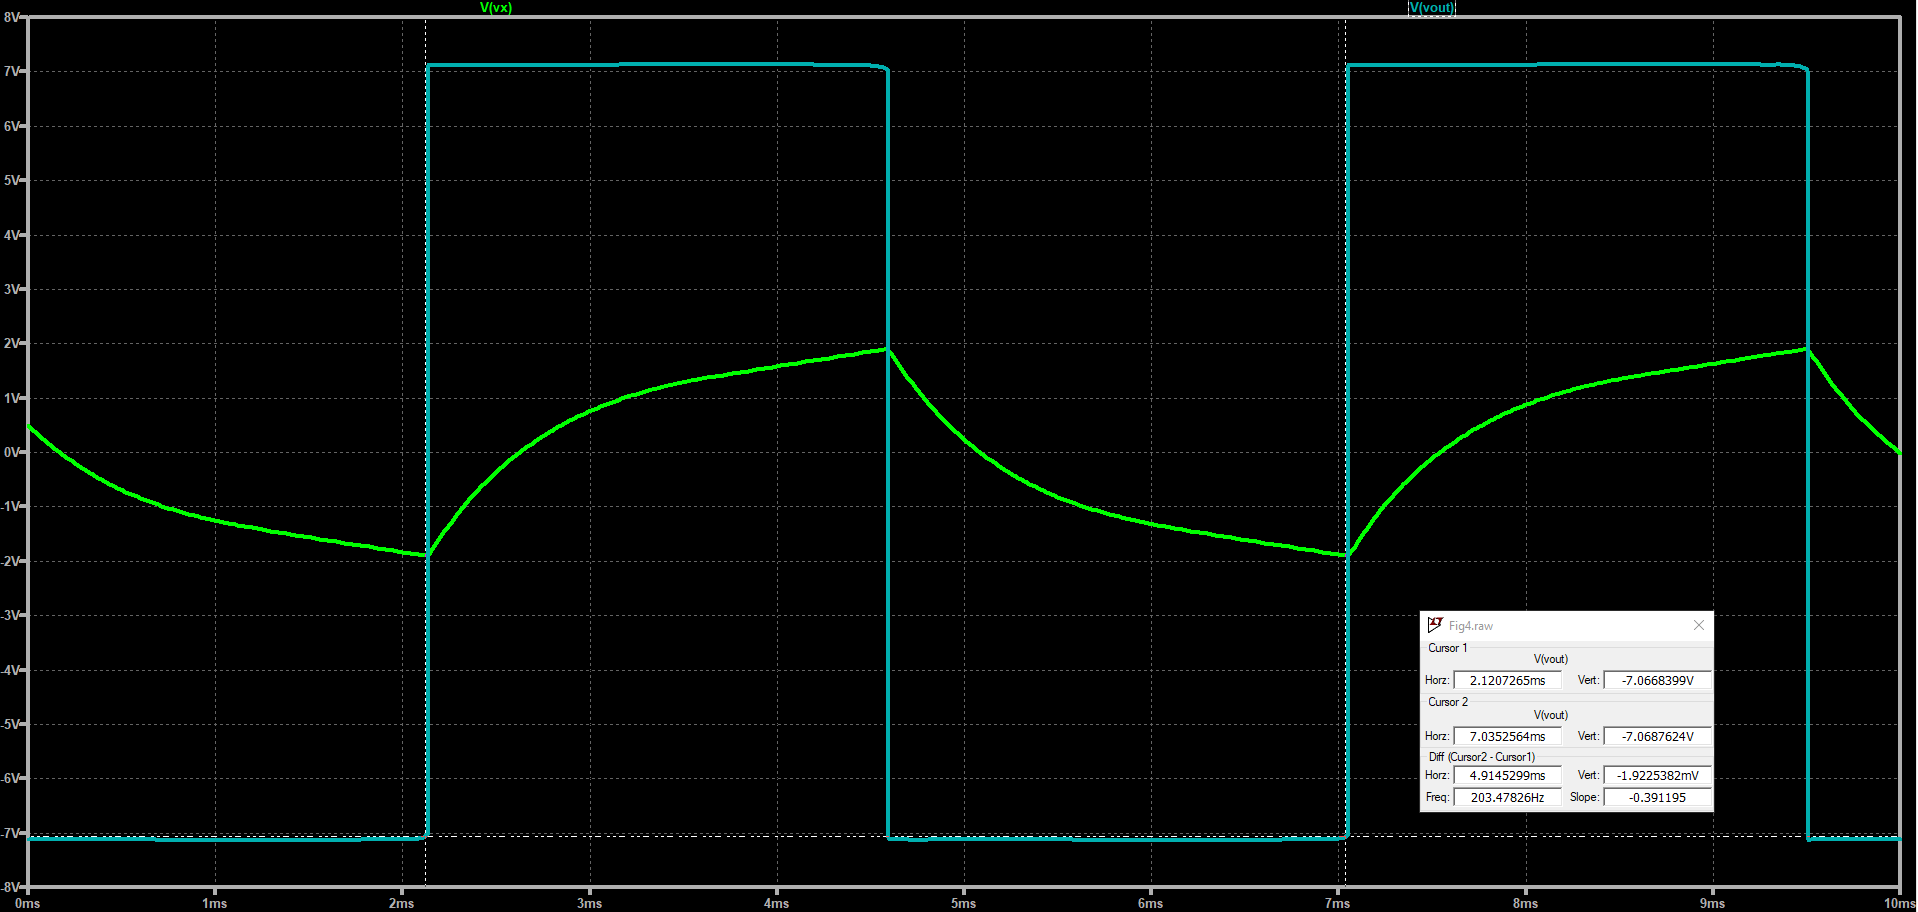
\includegraphics[width=0.86\textwidth]{4bC100R100.png}
        \caption{$v_c(t)$ (green) and $v_{out}(t)$ (cyan) for $C = 100nF, R_3 = 100k\Omega$}
        \label{Fig:4bC100R100}
    \end{figure} \\
    The waveforms for $v_c(t)$ and $v_{out}(t)$ for $C = 100nF, R_3 = 10k\Omega$ can be seen in Figure \ref{Fig:4bC100R10}. The period was measured to be approximately 915$\mu$s (1.09 kHz).
    \begin{figure}[h!]
        \centering
        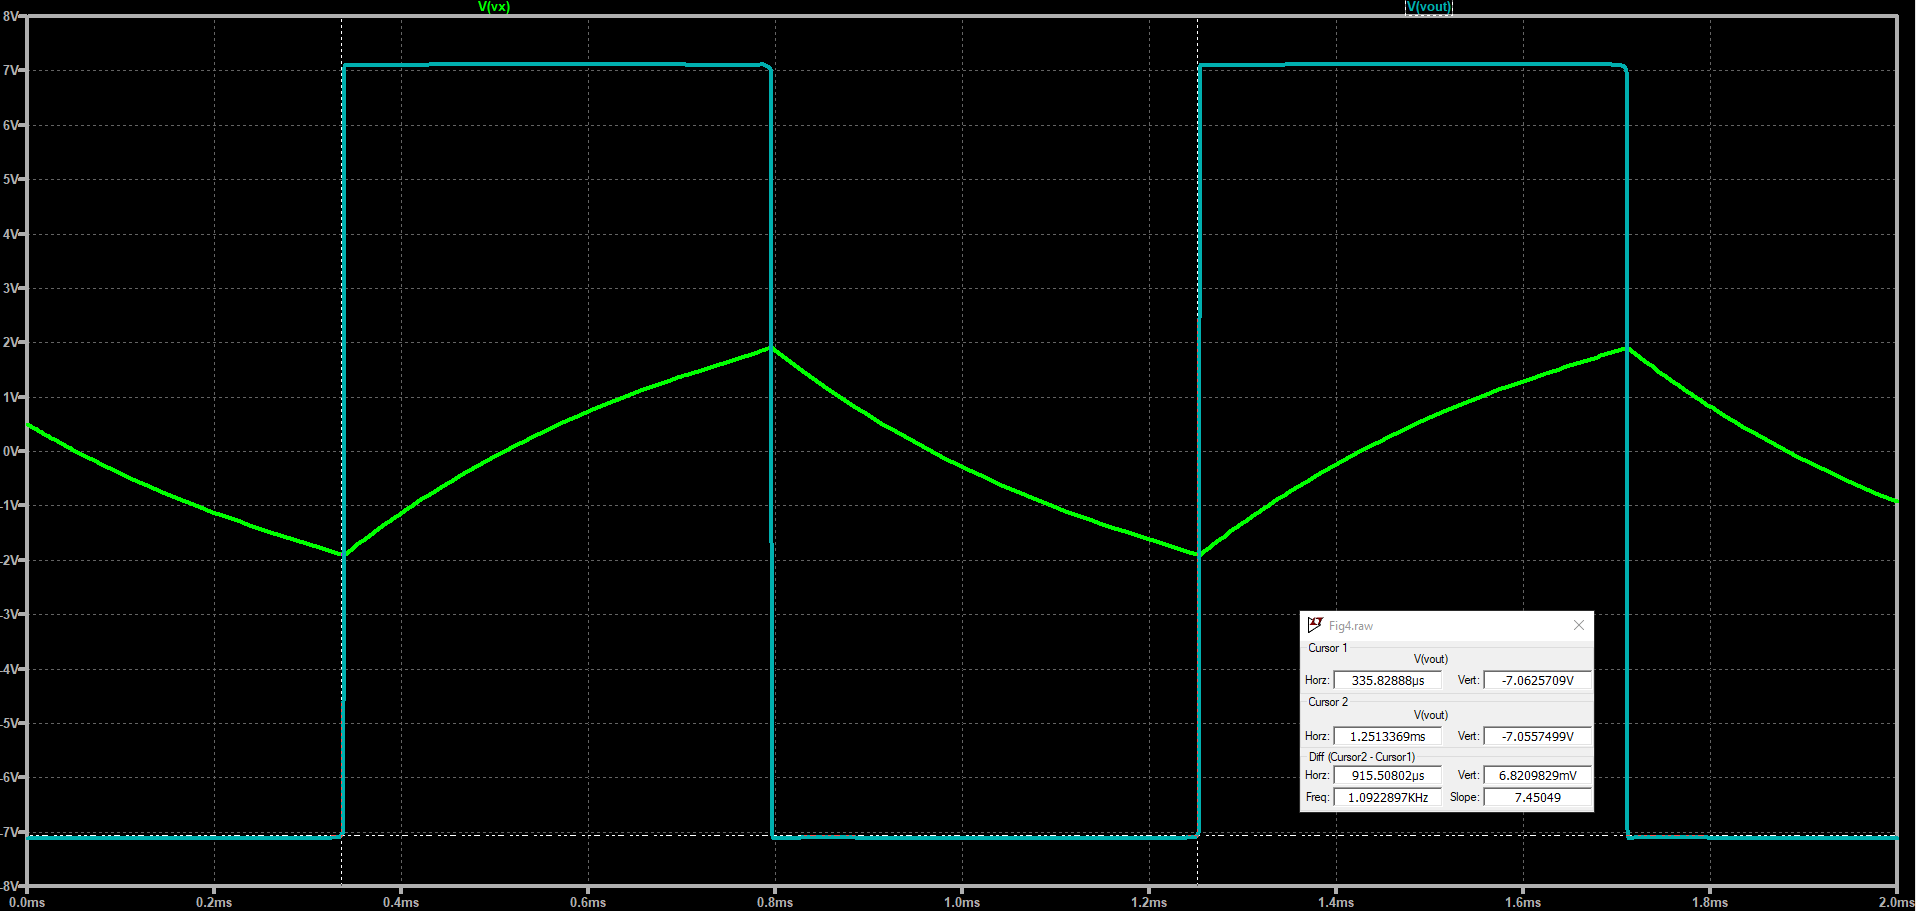
\includegraphics[width=0.86\textwidth]{4bC100R10.png}
        \caption{$v_c(t)$ (green) and $v_{out}(t)$ (cyan) for $C = 100nF, R_3 = 10k\Omega$}
        \label{Fig:4bC100R10}
    \end{figure} \pagebreak
    \item The waveforms for $v_c(t)$ and $v_{out}(t)$ can be seen in Figure \ref{Fig:4c}. The period was measured to be approximately 310$\mu$s (3.22 KHz).
    \begin{figure}[h!]
        \centering
        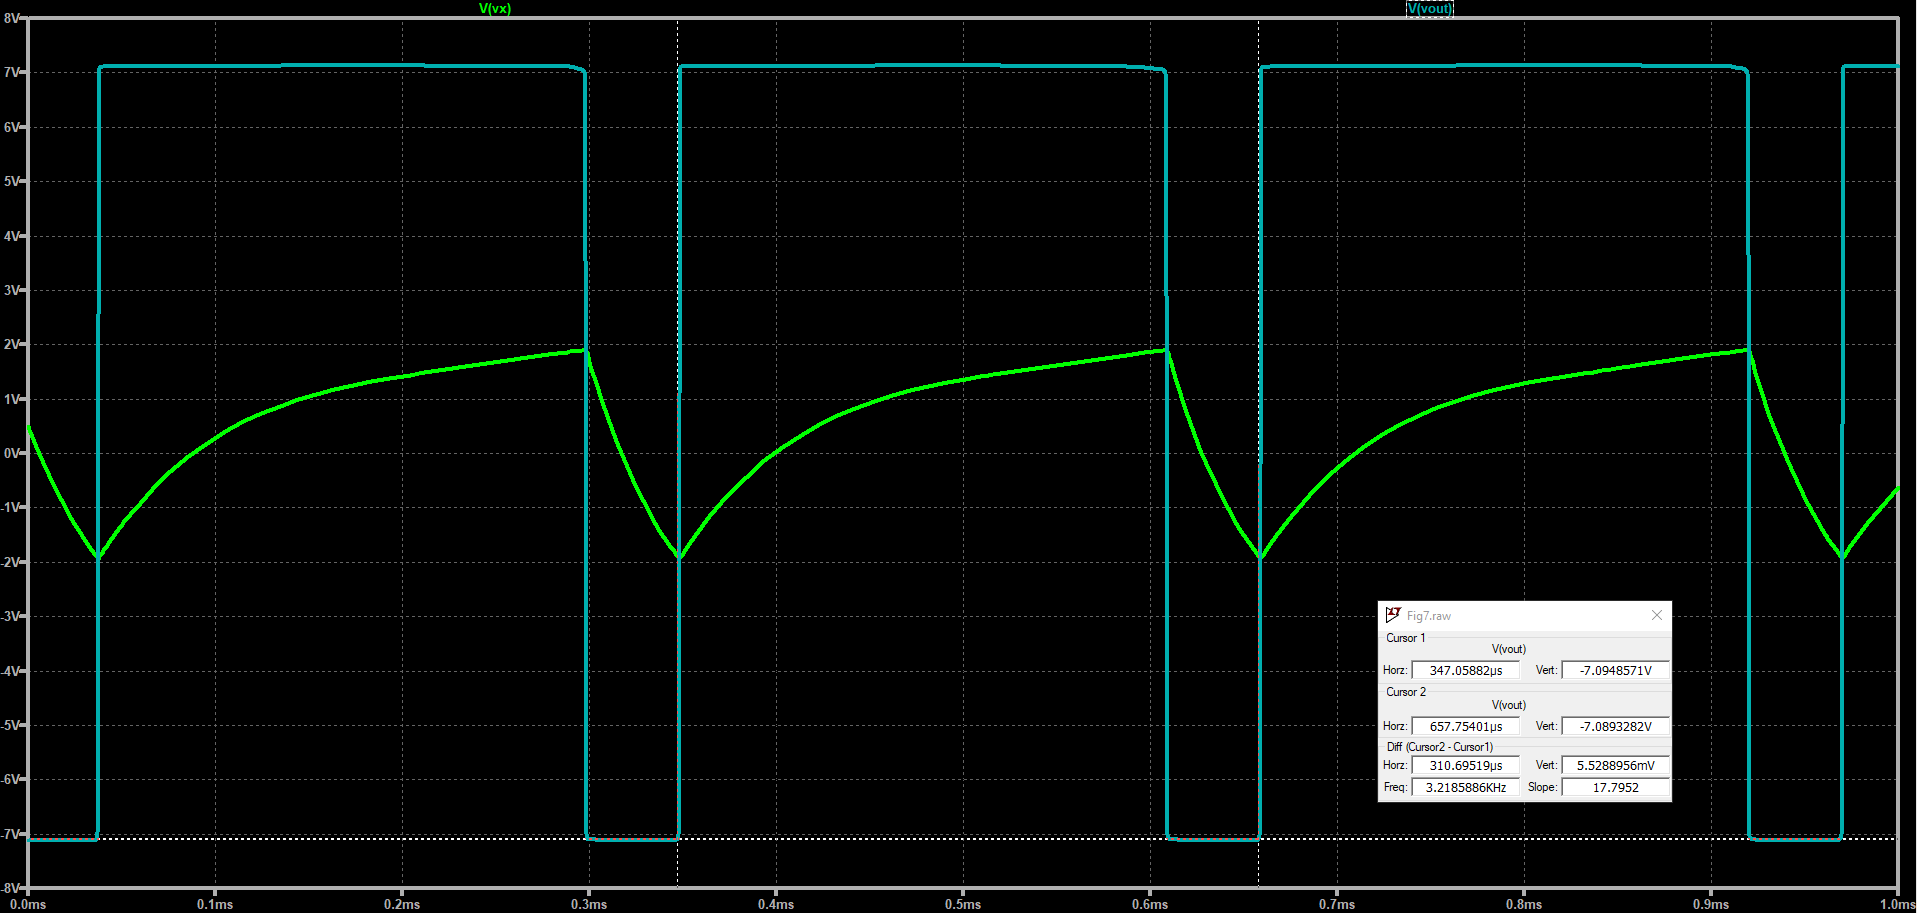
\includegraphics[width=0.86\textwidth]{4c.png}
        \caption{$v_c(t)$ (green) and $v_{out}(t)$ (cyan)}
        \label{Fig:4c}     
    \end{figure}
    
\end{enumerate}
\end{document}